% !TeX root = ../../../book.tex
\subsection{证明``$\subseteq$''}

回顾子集的定义,后续讨论中将频繁使用:

\begin{definition}
    给定集合 $A$ 和 $B$,若 $A$ 的每个元素也是 $B$ 的元素,则称 $A$ 是 $B$ 的\dotuline{子集}。
\end{definition}

\clearpage

假设需要证明如下命题:
\begin{center}
    设 $A$ 为集合……,$B$ 为集合……,证明 $A \subseteq B$。
\end{center}
如何利用子集的定义进行证明?直观理解是验证``$A$ 的每个元素也是 $B$ 的元素'',但不可仅凭此断言作为结论。关键在于严格证明 $A$ 的任意元素必然属于 $B$。此时``\textbf{任意固定}''这一表述将发挥重要作用。

\subsubsection*{``任意固定''}

如何同时处理 $A$ 的\emph{所有元素}?若 $A$ 仅有有限个元素(如 $3$ 个),或可逐项验证;但当 $A$ 含 $100$ 个、$100$ 万个乃至\emph{无穷}多个元素时,如何系统性地完成证明?

解决方案是引入 $A$ 的一个\textbf{任意固定}元素。其\textbf{任意性}体现在:除属于 $A$ 外,不附加任何特殊假设;其\textbf{固定性}表现为:赋予该元素特定名称(如 $a$, $x$, $t$),并在后续证明中始终指向同一对象。若能证明此元素属于 $B$,即同时证得 $A$ 的\emph{所有}元素均属于 $B$。

\subsubsection*{示例}

让我们通过具体案例理解上述过程。以下展示命题陈述、证明思路分析及正式证明。

\begin{lemma}\label{lemma3.9.1}
    设 $A,B,X$ 为任意集合。若 $X \subseteq A$ 且 $X \subseteq B$,则 $X \subseteq A \cap B$。
\end{lemma}

\emph{直观理解}:通过维恩 (Venn) 图分析。$X \subseteq A$ 与 $X \subseteq B$ 同时成立时,$X$ 必然完全位于 $A$ 与 $B$ 的重叠区域内,即 $A \cap B$ 所表示的区域。这佐证了命题的正确性,但并非严格证明!
\begin{center}
    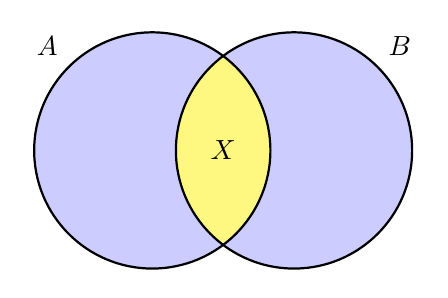
\begin{tikzpicture}[thick, set/.style = {circle, minimum size = 3cm, fill=blue!20}]

        % Set A
        \node[set,label={135:$A$}] (A) at (0,0) {};

        % Set B
        \node[set,label={45:$B$}] (B) at (1.8,0) {};

        % Intersection
        \begin{scope}
            \clip (0,0) circle(1.5cm);
            \clip (1.8,0) circle(1.5cm);
            \fill[yellow!50](0,0) circle(1.5cm);
        \end{scope}

        % Circles outline
        \draw (0,0) circle(1.5cm);
        \draw (1.8,0) circle(1.5cm);

        % Set intersection label
        \node at (0.9,0) {$X$};
    \end{tikzpicture} 
\end{center}

为了证明这个命题,我们引入任意固定元素 $x \in X$。关于它我们知道什么?假设 $X \subseteq A$。符号``$\subseteq$''的定义表明 $X$ 的所有元素都属于 $A$。既然 $x$ 是 $X$ 的元素,那么 $x$ 也属于 $A$。这很方便!类似地,由 $X \subseteq B$ 可得 $x \in B$。综上,我们利用``$\cap$''的定义推知 $x \in A \cap B$。很好!现在将其形式化。

\begin{proof}
    设 $x \in X$ 为任意固定元素。

    假设 $X \subseteq A$,根据 $\subseteq$ 的定义,可得 $x \in A$。

    同理,由 $X \subseteq B$,可得 $x \in B$。

    因为 $x \in A$ 且 $x \in B$,根据 $\cap$ 的定义,这意味着 $x \in A \cap B$。

    综上,对任意 $x \in X$ 均有 $x \in A \cap B$。由于 $x \in X$ 是任意的,因此 $X \subseteq A \cap B$。
\end{proof}

下面看一个稍复杂的例子。

\begin{proposition}
    设 $A$ 和 $B$ 为任意集合。则 $\mathcal{P}(A) \cap \mathcal{P}(B) \subseteq \mathcal{P}(A \cap B)$。
\end{proposition}

这成立吗?回顾 \ref{sec:section3.5} 节习题 \ref{exc:exercises3.5.6} 中的具体示例可知,该命题具有一般性。下面证明其正确性。

\emph{直观理解}:此命题涉及多层次的定义,尤其需注意幂集运算。关键点在于理解 $\mathcal{P}(A)$ 是 $A$ 的所有子集的集合。待证子集关系表明:无论 $\mathcal{P}(A) \cap \mathcal{P}(B)$ 的具体形式如何(稍后分析,但眼下你需要意识到它是一个集合),它都是 $\mathcal{P}(A \cap B)$ 的子集。这一观察将引导后续证明的框架。

无需显式计算 $\mathcal{P}(A) \cap \mathcal{P}(B)$,证明可从``设 $X \in \mathcal{P}(A) \cap \mathcal{P}(B)$ 为任意集合''开始。因为根据``$\subseteq$''的定义,需要证明该集合的任意元素也属于 $\mathcal{P}(A \cap B)$。这确定了证明的\textbf{结构}。

元素 $X \in \mathcal{P}(A) \cap \mathcal{P}(B)$ 是什么?它是集合,且同时属于 $\mathcal{P}(A)$ 和 $\mathcal{P}(B)$。下面直接给出正式证明,但建议你先尝试自行证明。完成后可与下文比较,检验步骤的完整性和表述的清晰性。

\begin{proof}
    设 $X \in \mathcal{P}(A) \cap \mathcal{P}(B)$ 为任意固定集合。

    根据 $\cap$ 的定义,有 $X \in \mathcal{P}(A)$ 且 $X \in \mathcal{P}(B)$。

    因为 $X \in \mathcal{P}(A)$,根据幂集的定义,可知 $X \subseteq A$。

    同理,因为 $X \in \mathcal{P}(B)$ 可知 $X \subseteq B$。

    因为 $X \subseteq A$ 且 $X \subseteq B$,由引理 \ref{lemma3.9.1} 可得 $X \subseteq A \cap B$。

    因为 $X \subseteq A \cap B$,根据幂集的定义,可得 $X \in \mathcal{P}(A \cap B)$。

    由于 $X$ 是任意固定集合,因此可得 $\mathcal{P}(A) \cap \mathcal{P}(B) \subseteq \mathcal{P}(A \cap B)$。
\end{proof}

你的证明与上述一致吗?是否引用了前述引理?或无意中重复证明了已有结论?请记住:证明的重要价值在于结论的可复用性!尽管在证明中重复证明先前结论并无技术错误,但直接引用可以极大节省精力。若解题时产生``似曾相识''的感觉,不妨回溯相关定理或引理,利用已有结论提升效率。
